\documentclass[]{article}

\usepackage[pdftex]{graphicx}
\usepackage[top=1in, bottom=1in, right=1.25in, left=1.25in]{geometry}
\usepackage{hyperref}

\begin{document}

	\setlength{\parindent}{0pt}
	\setlength{\parskip}{6pt}

	% Title Page
	\begin{titlepage}



		\title{\textbf{Proposed Design Report}}
		\author{BU ProPANE Team:\\Griffin Dunn\\Colin Madigan\\Phillip Stahlfeld}
		\date{November 29, 2012}
		\maketitle



		\noindent
		The purpose of this report is to present the design the BU ProPANE team will be implementing and testing in the upcoming semester. The report includes a design overview, design specifics, budget, and tentative schedule for the spring semester. The schedule will include a list of demonstrations to be completed while working towards Version 1.0 of the ProPANE system. 
		\thispagestyle{empty}
		
		
		
	\end{titlepage}
	
	
	
	
	% Begin  Real  Document
	\pagenumbering{roman}
	\tableofcontents
	\newpage
	
	\pagenumbering{arabic}
	\setcounter{page}{1}
	\thispagestyle{empty}
	
	\section{Design Overview}
		The goal of this section is to provide a high-level overview of the proposed design for the BU ProPANE system. It provides a view of the approach to the problem without diving into implementation level details. 
		
		\subsection{Concept of Operation}
			As mentioned in previous documentation concerning this project (found here: \url{http://sites.google.com/site/bupropane}), the ProPANE system will be broken down into the capture system and the analysis system. The purpose of the capture system is to collect images of a whiteboard throughout the course of a normal class. The purpose of the analysis system is to process these images for the purpose of generating key images. Figure \ref{img:concept-of-operation} shows the concept of operation for the system. There can be multiple capture systems that send images to a single analysis system for processing. 
			
			\begin{figure}[h]
				\centering
				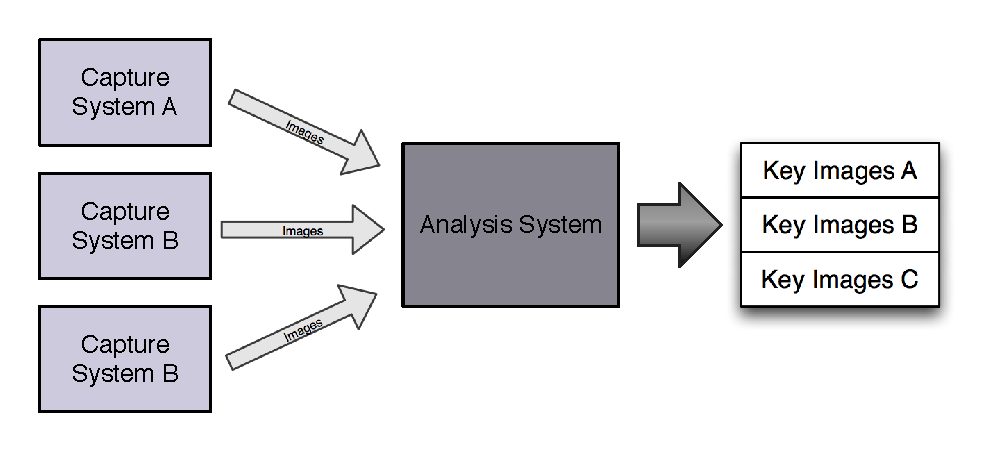
\includegraphics[scale=0.8]{images/concept-of-operation.eps}
				\caption{This figure shows the concept of operation for the overall ProPANE system. Capture systems capture images of whiteboards and send the images to the analysis system. The analysis system processes the images and generates the key images that the user desires.}		
				\label{img:concept-of-operation}
			\end{figure}
		
		\subsection{Capture System Overview}
			The capture system is a camera mounted on a tripod facing the whiteboard where information is to be captured. This setup can be seen in Figure \ref{img:setup-capture-system}. The camera will be installed with a piece of software that will take pictures periodically throughout the course of a lecture and save them to a local storage medium. These collected images can then be transferred to the analysis system for generating the desired key images. 
			
			\begin{figure}[h]
				\centering
				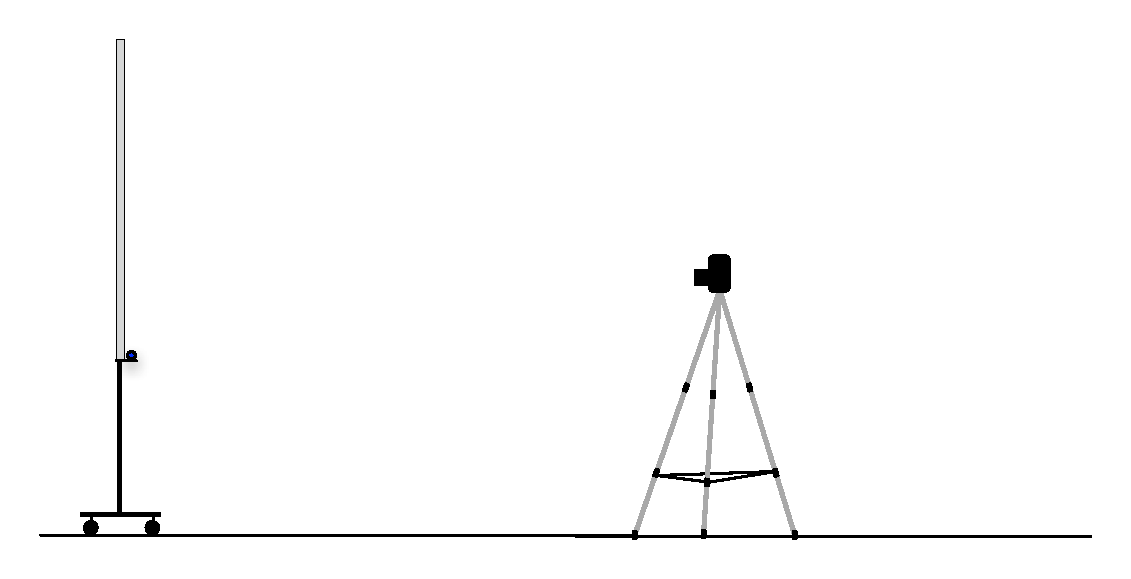
\includegraphics[scale=0.8]{images/setup-capture-system.eps}
				\caption{This figure shows the setup for the capture system with the camera on a tripod facing the whiteboard where the professor will be lecturing. Note that the capture system could be placed on a desk or table depending on the desired tripod.}		
				\label{img:setup-capture-system}
			\end{figure}
		
			
		
	\section{Capture System}
		The capture system is composed of capture device and capture stand. The BU ProPANE team has decided to use the Samsung Galaxy Camera for the capture device and the INSERT STAND HERE. 
			
			\subsection{Camera}
				The Samsung Galaxy Camera is an Android-based point-and-shoot digital camera. This device was selected for the project because it met the required criteria better than the other cameras that were examined. 
				
				\subsubsection{Camera Criteria}
					The following is a list of criteria that the camera had to meet based on the requirements documented in the technical specifications for this project:
					\begin{itemize}
						\item Programmable to allow for automatic, repetitive captures
						\item Battery capacity to allow for a full lecture of captures
						\item Portable to allow for transportation between rooms
						\item High enough resolution to discern characters within specified operating distance
					\end{itemize}
				
				\subsubsection{Camera Comparisons}
					After coming across a Microsoft Research paper documenting a solution to an extremely similar whiteboard problem, the initial idea was to use the same approach as the Microsoft team and connect a camera via USB to a computer that would signal for the camera to take a picture. Conferring with the clients resulted in this idea violating the programmable requirement for the camera because the clients desired a wireless solution. 
					
					Further research into programmable cameras resulted in the discovery of several Android-based cameras. Of the cameras on the market during the research period (beginning of October 2012), the Nikon Coolpix S800 was the forerunner since---according to user reviews---it provided the most suitable interface for programming. However, further research into the camera revealed that the battery for the camera was only capable of taking approximately 150 shots per charge. For a 52 minute class, the camera will be required to take at least 624 pictures (i.e. one picture every five seconds).
					
					Continued research yielded an advertisement for the Samsung Galaxy Camera. The Samsung Galaxy Camera has a greater programmability, larger battery (7 hours), and higher resolution than the Nikon Coolpix S800.
				
			\subsection{TRIPOD}
			
			
			\subsection{Application}
				Since the Samsung Galaxy Camera runs Android 4.1 Jelly Bean, the capture system will be based around an Android application. The Android API has an interface for cameras that let the programmer perform actions such as: taking a picture, autofocusing the camera, and saving the resulting picture as a JPEG. The following sections document the proposed design for the application.
				
				\subsubsection{Graphical Layout}
					The layout for the system was designed to separate the configuration of a capture from the capture itself. The initial screen that the user will see is Figure \ref{img:app-main-layout} where he will be able to configure how often pictures will be taken and the name of the directory where pictures will be stored (the name of the capture). Once the user clicks on the "Continue" button, he will be taken to the screen seen in Figure \ref{img:app-preview-layout} where he will be able to adjust the camera angle/focus/etc to capture the desired portions of a whiteboard. Once the ``Start Capture" button is clicked, the system will start capturing images. The ``Stop Capture" button will stop the system from capturing images and return it to the initial screen. 
					
					The first iteration of the capture system's interface was designated as a demonstration for this semester so it can be seen in Figure \ref{img:screenshot-app-preview}. Note that this is running on a Motorola Droid RAZR Maxx running Android 4.0 and has not been tested on the Samsung Galaxy Camera running Android 4.1. 
									
					\begin{figure}
						\centering
						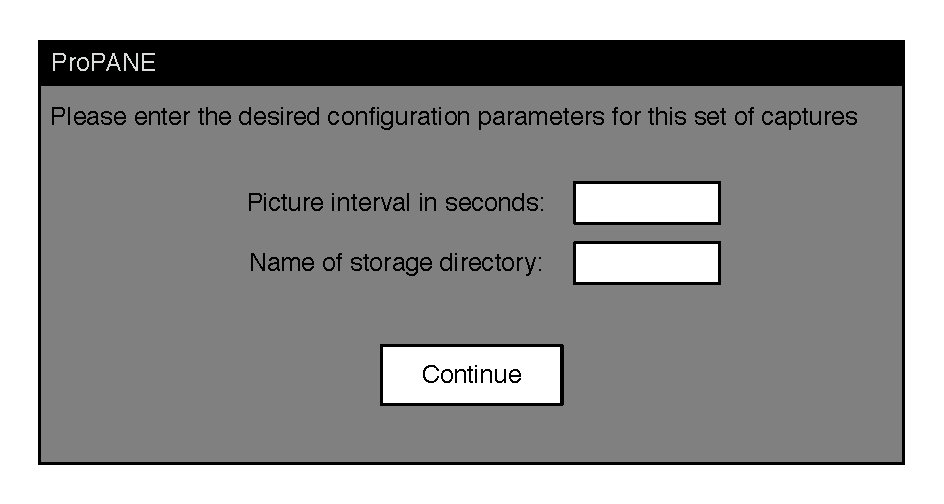
\includegraphics{images/app-main-layout.eps}
						\caption{This figure shows the planned layout for the capture system's initial screen/Android activity.}
						\label{img:app-main-layout}
					\end{figure}
					
					\begin{figure}
						\centering
						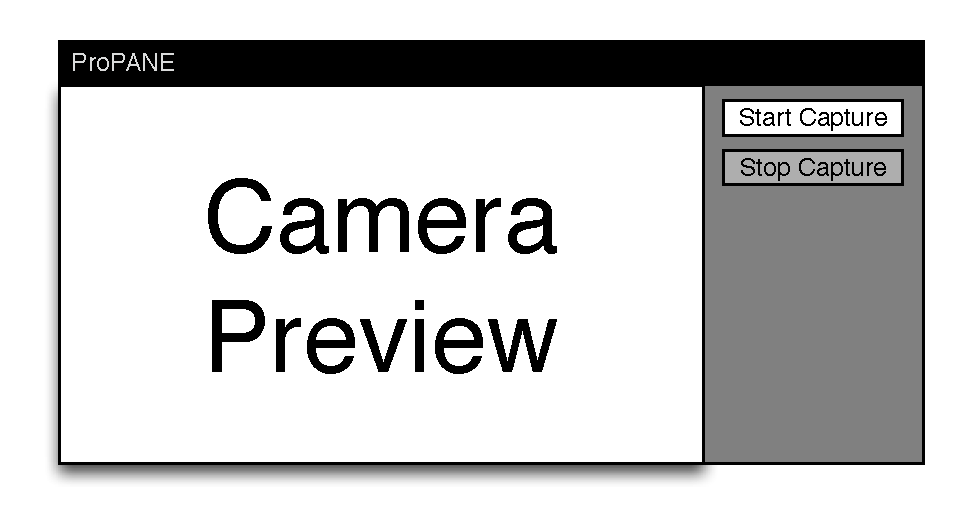
\includegraphics{images/app-preview-layout.eps}
						\caption{This figure shows the planned layout for the capture system's screen/Android activity that provides the ability to preview what part of the whiteboard will be captured by the system. Note that once the user clicks on the ``Start Capture" button, the ``End Capture" button will become enabled and the ``Start Capture" will become disabled.}
						\label{img:app-preview-layout}
					\end{figure}
					
					\begin{figure}
						\centering
						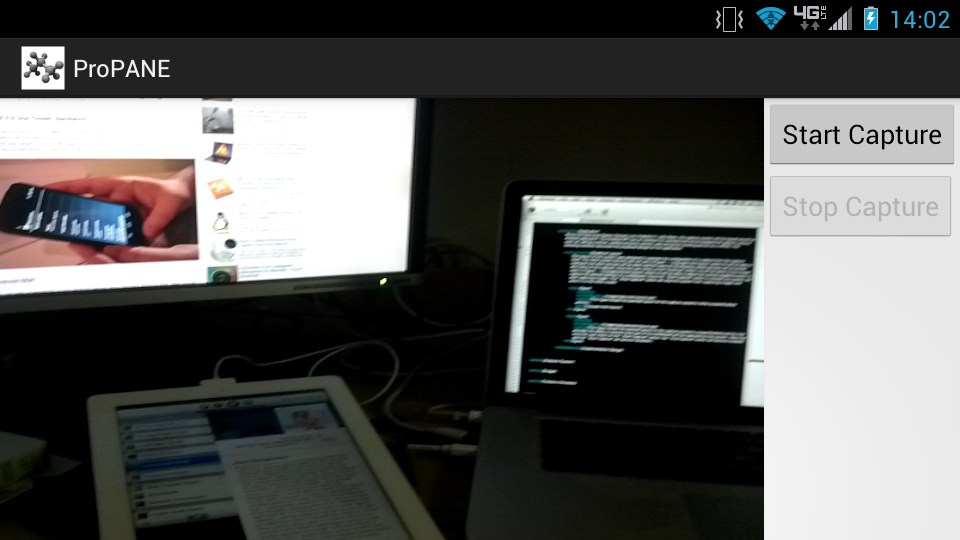
\includegraphics[scale=0.4]{images/screenshot-app-preview.png}
						\caption{This figure shows the first iteration of the app for the capture system}
						\label{img:screenshot-app-preview}
					\end{figure}
					
					
					
				\subsubsection{Class Design}
					For the full class diagram for the capture system app, see Figure \ref{img:uml-capture-system}. The main classes to focus on are MainScreen and PreviewScreen because they represent the two screen that will be shown to the user. The Preview class is just used to display what the camera is currently viewing.
					
					The MainScreen is responsible for creating the initial interface that the user sees (Figure \ref{img:app-main-layout}), collecting the necessary input from the user (picture interval, storage directory), sending that information to the PreviewScreen, and starting the PreviewScreen Activity. The design for the MainScreen will be done using the standard I/O classes provided by the Android SDK since it does not require a special component (such as a preview for the camera). Sending the input to the PreviewScreen activity will be accomplished through the use of Android Intents, which are designed to start new Activities and pass those Activities values from the creator. The ProPANE team has completed the Intents tutorial on the \url{http://developer.android.com} site demonstrating that they are capable of implementing this portion of the design. 
					
					The PreviewScreen is responsible for showing the user a preview of what to capture and creating an interface for starting/stopping the capture. When the user presses the ``Start Capture" button, the Activity will start a Service that autofocuses the camera and repeatedly takes pictures at the specified interval until the ``Stop Capture" button is pressed. The Service is needed because the capturing must still be happening when the screen goes to sleep. This is necessary to save battery power on the Samsung Galaxy Camera by putting the screen to sleep during the hour long captures. The Preview SurfaceHolder seen in the class diagram is the component that connects the PreviewScreen to the output from the camera. This feature is currently functional in the demonstration app as seen in Figure \ref{img:screenshot-app-preview}. 
					
					\begin{figure}
						\centering
						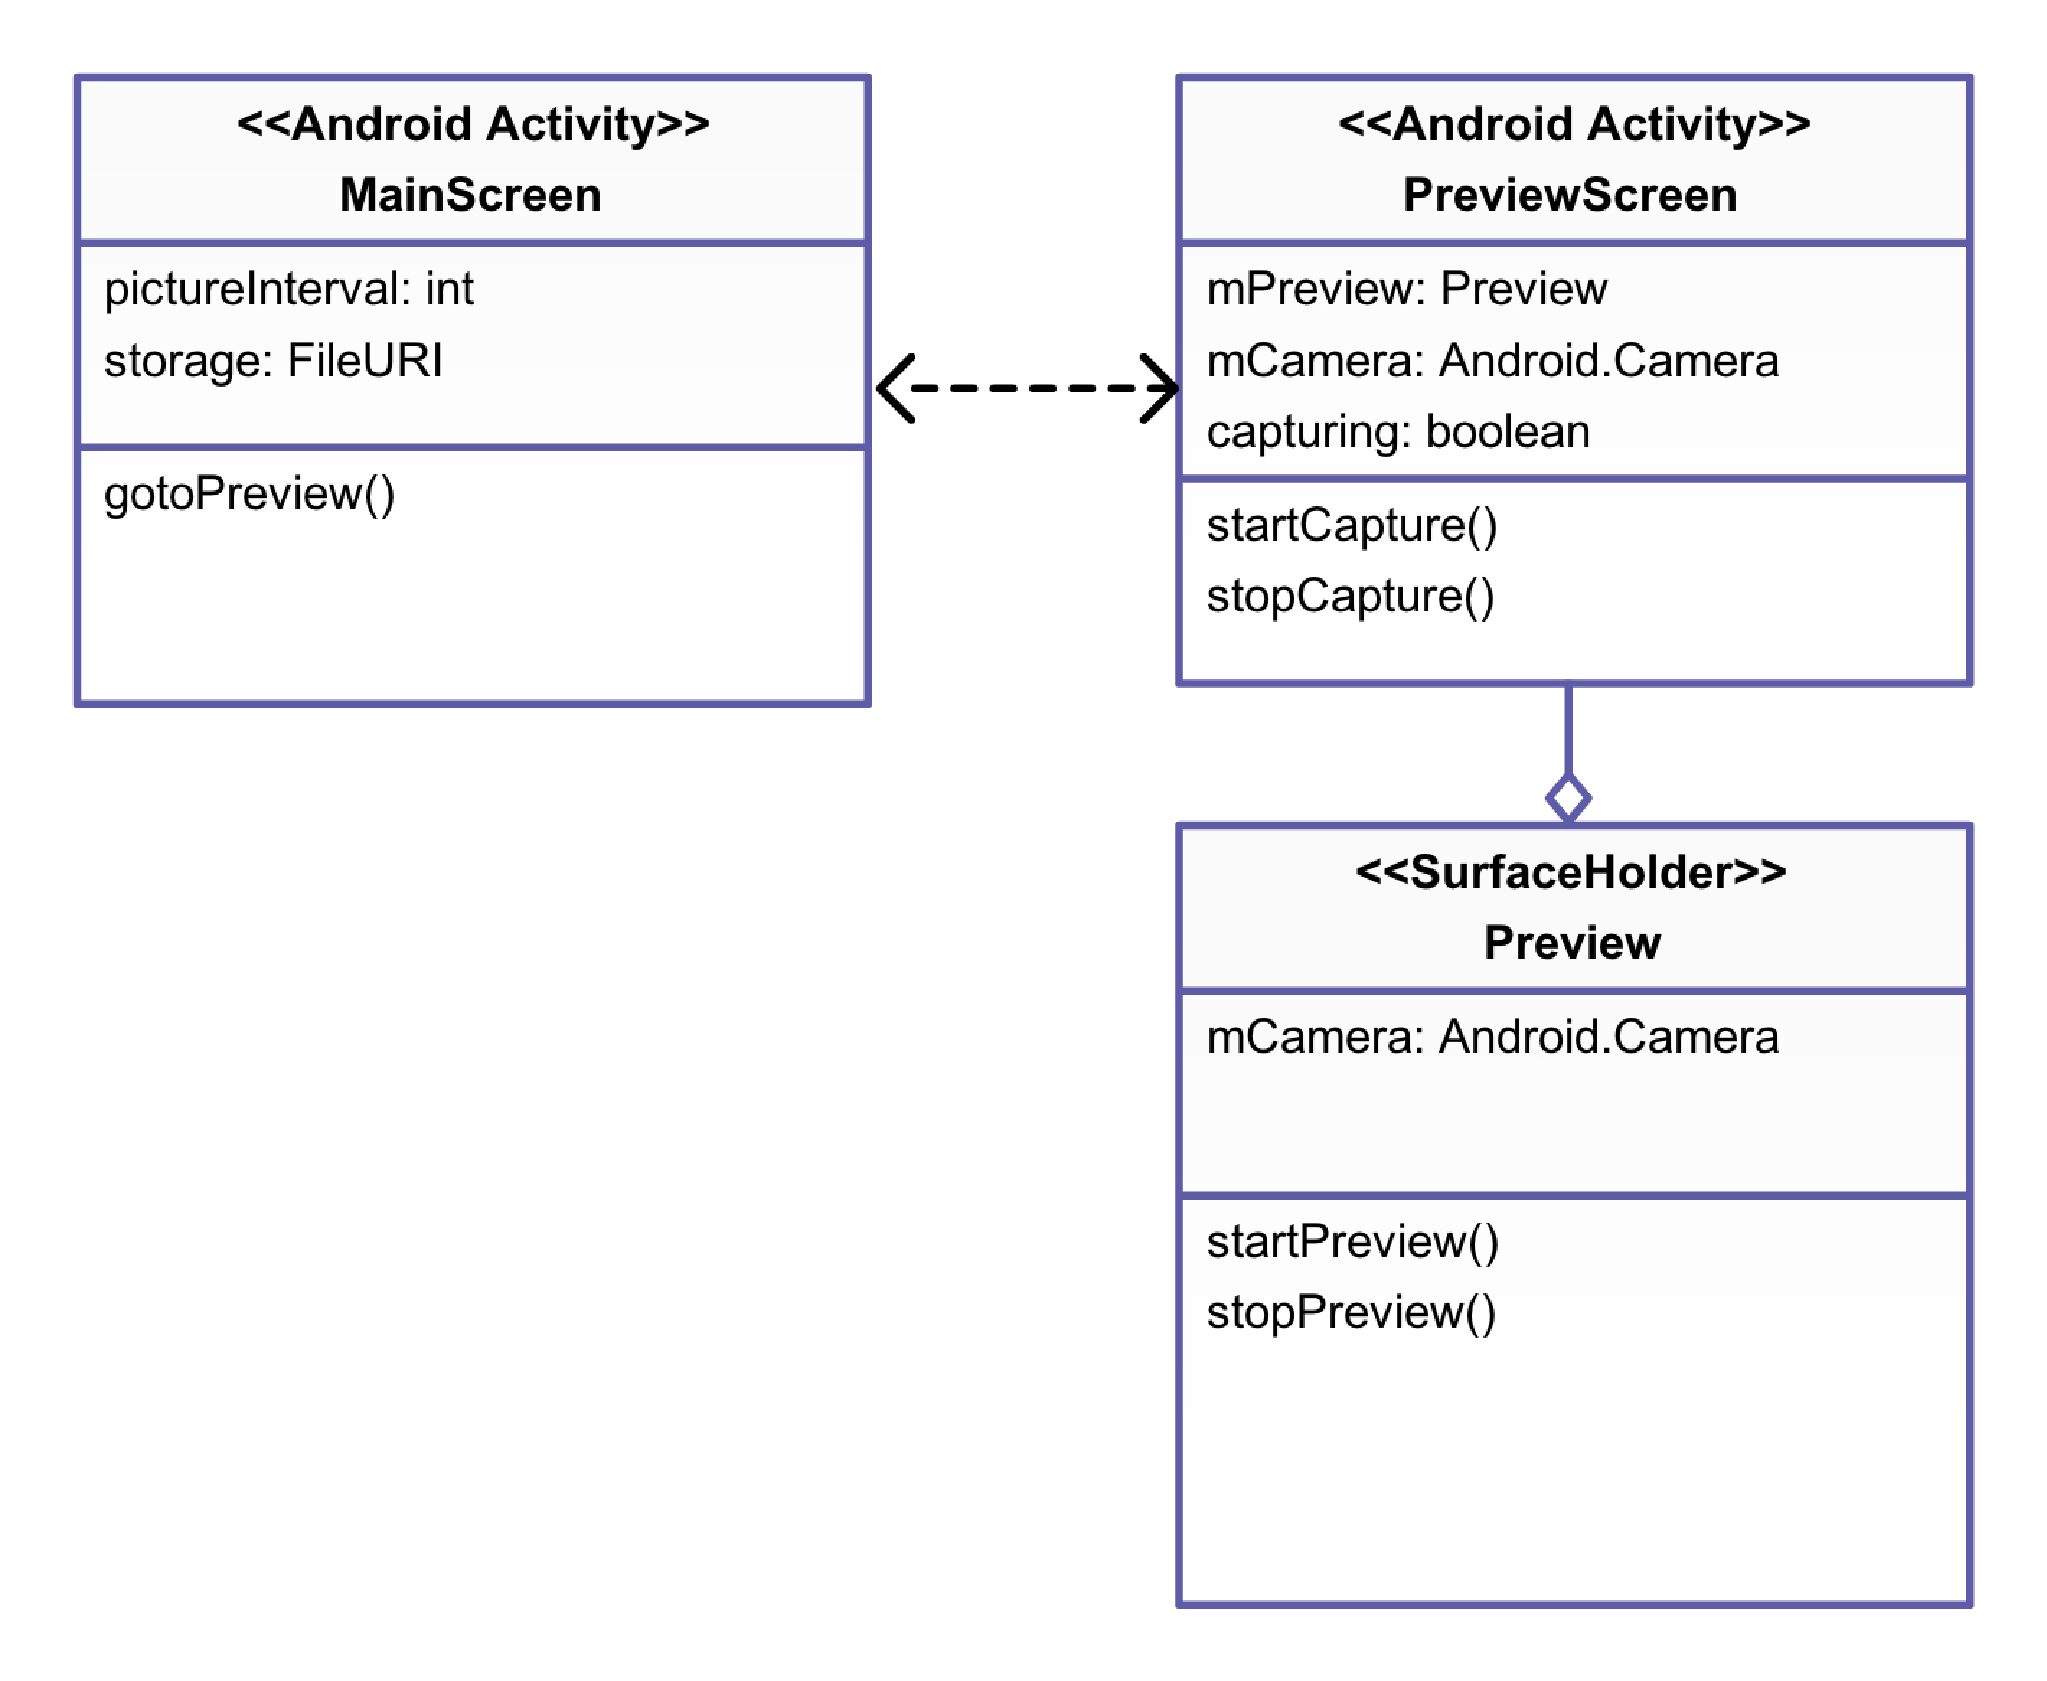
\includegraphics[scale=0.3]{images/uml-capture-system.pdf}
						\caption{This figure shows the class diagram for the Android based capture system app}
						\label{img:uml-capture-system}
					\end{figure}
					
					
		
	
	\section{Analysis System}
	
	
	\section{Budget}
	
	
	\section{Tentative Schedule}
		
		
		
			
\end{document}